\chapter{Modellierung}\label{cha:modell}

In diesem Kapitel wird die Modellierung des Gesamtsystems erläutert und auf dessen Implementierung in \ml\ und \Simulink\ eingegangen.

\section{Modell des \spd-Systems}\label{sec:spdModell}


Die Modellierung des \spd-Systems orientiert sich zunächst an den Modellen der vergangenen Arbeiten. 
Diese bezogen sich auf die Herleitung von \cite{modpen}. 
Dabei gibt es die Variante \emph{Kraftsystem}, das als Eingang die Kraft annimmt, welche am Schlitten wirkt, sowie das vereinfachte \emph{Beschleunigungssystem}, das direkt die Beschleunigung des Schlittens als Eingang erhält.


%\begin{figure}[bp]
	%\centering
		%\includegraphics[width=0.7\textwidth]{Bilder/intro.pdf}
	%\caption{Idee des zentralen Reglerentwurfs}
	%\label{fig:intro}
%\end{figure}

\begin{figure}[h]
	\centering
		\begin{tikzpicture}[scale=1, auto, >=stealth',x=1cm,y=1cm]

	\def\pu{30}
	\def\lu{3}
	\def\su{2}
	
	\def\po{50}
	\def\lo{2.5}
	\def\so{1}

	\draw[thick] (-1,-0.5) |- (1,0.5) |- cycle;
	
	%\path (0,0) ++(\pu+90:\su) coordinate (su);
	%\path (0,0) ++(\pu+90:\lu) coordinate (lu);
	
	
	\begin{scope}[rotate=\pu]
		\draw[fill=white,thick] (1mm,0) -- (1mm, \lu) arc[start angle=0, end angle=180, radius=1mm] 
						-- (-1mm, 0) arc[start angle=180, end angle=360, radius=1mm];
		\draw[] (0,0) circle[radius=0.5mm];
		\draw[fill=black] (0, \su) circle[radius=0.5mm];
		
		\path (0, \su) coordinate (su);
		\path (0, \lu) coordinate (lu);
		
		\draw[very thin] (-1.5mm, 0) -- (-7.5mm, 0);
		\draw[very thin] (-1.5mm, \su) -- (-3.5mm, \su);
		\draw[white, <->] (-3mm, 0) -- (-3mm, \su); 
		\draw[very thin, <->] (-3mm, 0) -- node[pos=0.75,inner sep=0pt]{$s_1$} (-3mm, \su);

		\draw[very thin] (-1.5mm, \lu) -- (-7.5mm, \lu);
		\draw[white, <->] (-7mm, 0) -- (-7mm, \lu); 
		\draw[very thin, <->] (-7mm, 0) -- node[pos=0.75,inner sep=0pt]{$l_1$} (-7mm, \lu);
	\end{scope}
	
	\begin{scope}[rotate=\po,shift={(lu)}]
		\draw[fill=white,thick] (1mm,0) -- (1mm, \lo) arc[start angle=0, end angle=180, radius=1mm] 
						-- (-1mm, 0) arc[start angle=180, end angle=360, radius=1mm];
		\draw[] (0,0) circle[radius=0.5mm];
		\draw[fill=black] (0, \so) circle[radius=0.5mm];
		
		\path (0, \so) coordinate (so);
		\path (0, \lo) coordinate (lo);
		
		\draw[very thin] (-1.5mm, 0) -- ++(-2mm, 0);
		\draw[very thin] (-1.5mm, \so) -- ++(-2mm, 0);
		\draw[white, <->] (-3mm, 0) -- (-3mm, \so); 
		\draw[very thin, <->] (-3mm, 0) -- node[pos=0.5,inner sep=0pt]{$s_2$} (-3mm, \so);
	\end{scope}

	\draw[thick,white,->] (0,1.8) arc[start angle=90, end angle=90+\pu, radius=1.8cm];
	\draw[thin,->] (0,1.8) arc[start angle=90, end angle=90+\pu, radius=1.8cm];
	\node at (90+\pu/2:1.5cm) {$\varphi_1$};
	\draw[thin,dashed] (0,0) -- (0, 2);
	
	\draw[thick,white,->] (lu) ++(0,1.8) arc[start angle=90, end angle=90+\po, radius=1.8cm];
	\draw[thin,->] (lu) ++(0,1.8) arc[start angle=90, end angle=90+\po, radius=1.8cm];
	\path (lu) +(90+\po/2:1.5cm) node {$\varphi_2$};
	\draw[thin,dashed] (lu) -- ++(0, 2);


	\node[anchor=south east] at (1,-0.5) {$m_0$};
	
	\draw[very thin] (90+\pu:0.9*\lu) -- ++(8mm,3mm) node[anchor=west] {$m_1$, $J_1$};
	\draw[very thin] ($(lu)!0.9!(lo)$) -- ++(-8mm,-3mm) node[anchor=east] {$m_2$, $J_2$};
	
	
	\draw[thin] (-1.5,-1) -- ++(0,-0.5);
	\draw[thin,->] (-1.5,-1.25) -- node{$x_0$} (0,-1.25); 
	
	\draw[thin,->] (-3,0) -- ++(0.5,0) node[anchor=south, inner sep=1pt]{\tiny $x$};
	\draw[thin,->] (-3,0) -- ++(0,0.5) node[anchor=west, inner sep=1pt]{\tiny $y$};
	
\end{tikzpicture}

			\caption{\dpd}
	 \label{fig:koord}
\end{figure}

\subsection{Koordinaten}

Das System aus Schlitten und Doppelpendel hat 3 Freiheitsgrade, die mit den \textbf{Minimal-\koor} 
\begin{align*}
	q_0 = x_0  \\
	q_1 = \varphi_1  \\
	q_2 = \varphi_2
\end{align*}
beschrieben werden. Die Koordinaten sind nach \figref{fig:koord} definiert.

Die Schwerpunktskoordinaten der Pendelstäbe ergeben sich zu
\begin{align*}
	\xe &= \xo - s_1 \sin{\phe}  \\
	\ye &=       s_1 \cos{\phe}  \\
	\xz &= \xo - l_1 \sin{\phe} - s_2 \sin{\phz}  \\
	\yz &=       l_1 \cos{\phe} + s_2 \cos{\phz}  \ .
\end{align*}


\subsection{Herleitung der Bewegungsgleichungen}

Um auf die \bwgl\ des Systems zu gelangen, wird in \cite{modpen} der \emph{Lagrange}-Formalismus verwendet. 
Dazu werden zunächst die kinetische und potentielle Energie des Gesamtsystems bestimmt sowie die nicht-konservativen Kräfte/Momente. 
Mit dem Formalismus ergeben sich die 3 \emph{gekoppelten} Bewegungsgleichungen für die Minimal-\koor. 
Um nach den zweiten Ableitungen aufzulösen, muss allerdings noch das \gls\ gelöst werden.

Die kinetische Gesamtenergie ergibt sich zu
	\[
	T = \einhalb m_0 \, \xop^2 + \einhalb m_1 (\xep^2+\yep^2) + \einhalb m_2 (\xzp^2+\yzp^2) + \einhalb J_1 \, \phep^2 + \einhalb J_2 \, \phzp^2
\]
und die potentielle Energie beträgt
	\[
	U = m_1\, g\, \ye + m_2\, g\, \yz  \ .
\]

Die nicht-konservativen Kräfte/Momente setzen sich aus der Antriebskraft $F$ am Schlitten (in~$\xo$-Richtung) und den Reibungs-Kräften/Momenten zusammen und lauten
\begin{align*}
	Q_0^* &= F + \Fd + \Fc  \\
	Q_1^* &= \Mde + \Mce - \Mdz - \Mcz  \\
	Q_2^* &= \Mdz + \Mcz
\end{align*}
mit den viskosen Dämpfungen
\begin{align*}
	\Fd  &= -d_0 \xop  \\
	\Mde &= -d_1 \phep  \\
	\Mdz &= -d_2 \left(\phzp-\phep\right)  \ .
\end{align*}

Die Berechnung der Ableitungen und das Lösen des \gls\ geschah bisher händisch, was im Allgemeinen fehleranfällig ist. 
In dieser Arbeit werden die \bwgl\ mithilfe der \textbf{symbolischen Toolbox} von \ml\ gelöst. 
Diese Vorgehensweise ist nicht nur weniger fehleranfällig, dadurch lässt sich das System auch sehr flexibel modifizieren.

Mit den obigen Gleichungen werden in \ml\ die für den \emph{Lagrange}-Formalismus benötigten Ableitungen symbolisch berechnet und das \gls\ mit dem symbolischen Solver gelöst und vereinfacht. 
Damit ergeben sich die \bwgl\ als Funktion der Minimal-\koor, der Systemparameter und des Eingangs.
\begin{align*}
	\xopp  &= f_{\xo}(\dots)  \\
	\phepp &= f_{\phe}(\dots)  \\
	\phzpp &= f_{\phz}(\dots)
\end{align*}


\subsection{\zrm}

Mit den \bwgl\ ergibt sich das eingangsaffine, \nlzrm\ mit Eingangsgröße $u=F$ wie folgt:
\begin{align}
	\vexp &= \ve{f}(\vex,u) = \ve{a}(\vex) + \ve{b}(\vex) \cdot F  \label{eq:zrm} \\\vspace{100cm}
	\ddt \begin{bmatrix}
		\xo \\ \xop \\ \phe \\ \phep \\ \phz \\ \phzp
	\end{bmatrix} &= \begin{bmatrix}
		\xop \\ a_2(\vex) \\ \phep \\  a_4(\vex) \\ \phzp \\  a_6(\vex)
	\end{bmatrix} + \begin{bmatrix}
		0 \\ b_2(\vex) \\ 0 \\  b_4(\vex) \\ 0 \\  b_6(\vex)
	\end{bmatrix} \cdot F
\end{align}

Beim Beschleunigungssystem gilt für den Eingang $u=\xopp=a$, womit die Schlittenbeschleunigung direkt vorgegeben und die Dynamik des Schlittens umgangen wird. 
Damit wird die erste der drei gekoppelten Bewegungsgleichungen ersetzt. 
Das geänderte \gls\ muss wieder gelöst werden und es ergibt sich das folgende \zrm:
\begin{align}
	\ddt \begin{bmatrix}
		\xo \\ \xop \\ \phe \\ \phep \\ \phz \\ \phzp
	\end{bmatrix} &= \begin{bmatrix}
		\xop \\ 0 \\ \phep \\  a_4(\vex) \\ \phzp \\  a_6(\vex)
	\end{bmatrix} + \begin{bmatrix}
		0 \\ 1 \\ 0 \\  b_4(\vex) \\ 0 \\  b_6(\vex)
	\end{bmatrix} \cdot a
\end{align}

Folgende Tabelle \ref{tab:abh} gibt Aufschluss über die Abhängigkeiten von Zuständen und \syp n. 
Grau hinterlegte Variablen sind nur im Kraftmodell vorhanden. 
Der Zustand \xo\ hat keinen Einfluss auf die Systemdynamik.
\begin{table}[h]
	\centering
		\begin{tabular}[t]{cc}
		\toprule
			Zustände	&	\textcolor{grey}{\xop}, \phe, \phep, \phz, \phzp	\\
			Geometrieparameter	&	$l_1$, $s_1$, $s_2$	\\
			Trägheitsparameter	&	\textcolor{grey}{$m_0$}, $m_1$, $m_2$, $J_1$, $J_2$ \\
			Reibungsparameter	&	\textcolor{grey}{$d_0$}, $d_1$, $d_2$, \textcolor{grey}{\Fco}, \Mceo, \Mczo, \textcolor{grey}{\xopth}, \pheth, \phzth	\\
			Umgebungskonstanten & $g$	\\
			\bottomrule
		\end{tabular}
	\caption{Abhängigkeiten von Zuständen und Parametern}
	\label{tab:abh}
\end{table}


Am Versuchsstand können die Schlittenposition und beide Pendelwinkel über Sensoren gemessen werden. Daher ergibt sich für den Ausgang beider Systeme
\begin{align}
	\ve{y} = \ve{h}(\vex)
	= \mat{C} \vex
	= \begin{bmatrix}
		1 & 0 & 0 & 0 & 0 & 0 \\
		0 & 0 & 1 & 0 & 0 & 0 \\
		0 & 0 & 0 & 0 & 1 & 0 
	\end{bmatrix} \vex
	= \begin{bmatrix}
		\xo \\ \phe \\ \phz
	\end{bmatrix}  \ .
	\label{eq:hx}
\end{align}
Es handelt sich demnach um ein \textbf{SIMO-System} (single input multiple output). 


\subsection{\crb}\label{sec:crb}

Da die \crb\ sowohl des Schlittens als auch der Pendelstäbe einen wesentlichen Einfluss zu haben scheint, darf diese nicht vernachlässigt werden. 
In den bisherigen Modellierungen wurde höchstens die \crb\ des Schlittens berücksichtigt. 
Da jedoch durch die Neukonstruktion des \dpd s die Messsignalübertragung (zur Vermeidung einer Kabelaufwickelung) über einen Schleifring realisiert wurde, besteht die Vermutung, dass dieser für eine erhöhte \crb\ verantwortlich ist. 
Dies würde das System bereits um einen sehr kleinen Arbeitsbereich nicht-linear machen, was die Regelung erschwert.

Im vorigen Projektseminar \cite{ribeiro} wurde die Reibung der Pendelstäbe mittels Identifikation ermittelt, aufgeteilt auf den viskosen und den Coulombanteil.

Die Formel der Gleitreibung lautet eigentlich 
	\[
	\Fc = \Fco  \cdot  \sign{\dot{x}} \ ,
\]
allerdings führt diese Implementierung aufgrund der \mrm{signum}-Funktion zu Komplikationen in der Simulation. 
Daher wird der Verlauf bei sehr niedrigen Geschwindigkeiten mit der $\tanh$ Funktion angenähert.
%In \cite{chang} und \cite{kisner} wurde die \crb\ mit der $\arctan$ Funktion modelliert.
%2/pi*atan(x0_p/x0_p_c2)

\begin{align}
	\Fc  &= -\Fco  \cdot \tanh{\left(\frac{\xop}{\xopth}\right)}  \\
	\Mce &= -\Mceo \cdot \tanh{\left(\frac{\phep}{\pheth}\right)}  \\
	\Mcz &= -\Mczo \cdot \tanh{\left(\frac{\phzp-\phep}{\phzth}\right)}
\end{align}

Dabei ist $\xopth$ gerade die Geschwindigkeit, bei der $\tanh(1)=0.7616$ von $\Fco$ erreicht ist.





\subsection{Ruhelagen}\label{sec:aps}

Die Ruhelagen \bzw \ap e eines nichtlinearen Systems ergeben sich aus
	\[
	\vexp_R = \ve{f}(\vex_R,u_R) = \ve{0}  \ .
\]
Für das \spds\ gibt es aufgrund der Periodizität von Sinus und Kosinus theoretisch unendlich viele Ruhelagen. Es werden daher die folgenden 4 prinzipiell unterschiedlichen betrachtet:
\begin{table}[h]
	\centering
		\begin{tabular}{lllllllll}
		\toprule
			\ap  & $u$ & \xo & \xop & \phe & \phep & \phz & \phzp & Stabilität  \\
			\midrule
			1	&	0 &	\xor	&	0	&	\pii	&	0	&	\pii	&	0	& stabil  \\
			2	&	0 &	\xor	&	0	&	\pii	&	0	&	0			&	0	& instabil  \\
			3	&	0 &	\xor	&	0	&	0			&	0	&	\pii	&	0	& instabil  \\
			4	&	0 &	\xor	&	0	&	0			&	0	&	0			&	0	& instabil  \\
			\bottomrule
		\end{tabular}
	\caption{Arbeitspunkte}
	\label{tab:aps}
\end{table}

Die Schlittenposition \xo\ ist dabei beliebig, da der Schlitten an jeder Position eine Ruhelage annehmen kann.
Die Reihenfolge der \ap e entspricht den Pendelpositionen \qq{von unten nach oben}.


%Position des Schlittenmittelpunktes x m −0,8 ≤ x ≤ 0,8
\section{Motor-Modell}

Das Motormodell besteht aus den drei Baugruppen Spannungs-Strom-Wandler, Gleichstrommotor und Getriebe. Die Modellierung der Baugruppen basiert auf den in Franke \cite{franke} erstmalig aufgestellten Gleichungen, die auch in den nachfolgenden Arbeiten zum Versuchsstand weiterhin angewendet wurden. Das Modell des Gleichstrommotors wird im Rahmen der vorliegenden Arbeit nun zusätzlich um die Berücksichtigung der Selbstinduktion des Motors erweitert.

Im Folgenden wird auf die mathematische Modellierung der drei Baugruppen näher eingegangen.

\subsection{Spannungs-Strom-Wandler}

Beim am Versuchsstand eingesetzten Spannungs-Strom-Wandler handelt es sich um einen Servoverstärker, der ursprünglich zur Drehzahlregelung von Gleichstrommotoren vorgesehen ist. Entsprechend folgt der pulsweitenmoduliert arbeitende Verstärker dem Prinzip einer übergeordneten Drehzahlregelung mit unterlagerter Stromregelung. Für die Anwendung am Versuchsstand ist der übergeordnete Drehzahlregelkreis jedoch aufgetrennt und in einen Spannungs-Strom-Wandler umfunktioniert worden. Dieser dient der Vorgabe eines konstanten Stromes durch Pulsweitenmodulation der Zwischenkreisspannung am Ausgang des Wandlers proportional zur Steuerspannung am Eingang. Das stationäre Verhalten kann aus diesem Grund durch einen Proportionalitätsfaktor $K_{UI}$ beschrieben werden
	\[
	I_{Motor} = K_{UI} \cdot U_{Steuer} .
\]

Gemäß Franke \cite{franke} lässt sich die Dynamik des Wandlers durch ein $PT_1$-Glied modellieren, sodass sich für den Wandler im Laplace-Bereich insgesamt die Gleichung
	\[
	I_{Motor}(s) = \frac{K_{UI}}{1+T_{UI}s} \cdot U_{Steuer}(s)
	\]
ergibt.


\subsection{Gleichstrommotor}

Bei dem verwendeten Motor handelt es sich um eine fremderregte Gleichstrommaschine, wobei die magnetische Erregung durch einen Permanentmagneten erzeugt wird \cite{franke}. Das elektromagnetische Drehmoment des Gleichstrommotors ist näherungsweise proportional zum Ankerstrom \cite{binder}. Hierbei wird vorausgesetzt, dass keine magnetische Sättigung vorliegt.
\[
	M_e = K_I \cdot I_a
\]

Neben dem elektromagnetischen Drehmoment sind außerdem parasitäre Reibmomente zu berücksichtigen. Die Modellierung der Reibung von Motor und Getriebe wird zusammen mit der Schlittenreibung in Kapitel \ref{sec:spdModell} behandelt. Ein rückwirkendes Moment durch die Federkraft des Riemens wird auf Grund der Annahme unendlicher Riemensteifigkeit vernachlässigt. 

Weiterhin wird das Drehmoment durch die Selbstinduktion des Motors geschwächt. Dieser Effekt ist in den Motormodellen von Franke \cite{franke} und den Nachfolgearbeiten bisher nicht berücksichtigt worden. Da die Erfahrung am realen Versuchsstand jedoch gezeigt hat, dass eine Modellierung der Selbstinduktion sinnvoll erscheint, wird diese im Rahmen dieser Arbeit in das Motormodell integriert.

Zum besseren Verständnis des Effekts wird zunächst das physikalische Prinzip der Selbstinduktion bzw. Gegeninduktion vergegenwärtigt. Fließt ein Strom durch den im Magnetfeld der Permanentmagneten ruhenden Anker des Motors, wirkt senkrecht zur Stromrichtung und zur Richtung des Magnetfeldes die Lorenzkraft auf die im Leiter der Ankerwicklung befindlichen Ladungsträger (Drei-Finger-Regel bzw. Rechte-Hand-Regel in technischer Stromrichtung). Es entsteht ein Drehmoment auf die Wicklung und der Anker beginnt sich zu drehen. Durch die Drehung bewegen sich die Ladungsträger nun zusätzlich zur Stromrichtung auch in Drehrichtung des Ankers. Auf diese Bewegungskomponente kann erneut das Prinzip der Lorentzkraft angewendet werden. Die resultierende zusätzliche Kraftkomponente, die in Abhängigkeit der Drehgeschwindigkeit auf die Ladungsträger wirkt, zeigt nun gegen die Stromrichtung (Lenzsche Regel). Auf Grund der Proportionalität zum Ankerstrom, wird das Drehmoment dadurch reduziert. 

Am Versuchsstand wird dieser induzierte Gegenstrom bei geringen Winkelgeschwindigkeiten des Motors durch den Stromregler des Spannungs-Strom-Wandlers ausgeregelt. Ab einer bestimmten Winkelgeschwindigkeit und einem konstantem Sollstrom ist der induzierte Gegenstrom größer als die Stellstromreserve, sodass er nicht mehr ausgeregelt werden kann. Nun nimmt der Strom und damit das Drehmoment mit steigender Winkelgeschwindigkeit ab bis die Leerlaufdrehzahl erreicht ist. 

ABBILDUNG I(w)-Kennlinie

Auf Grund der im Wandler integrierten Strombegrenzung zum Schutz von Motor und Verstärker ist der Stellstrom der Reglers zusätzlich begrenzt. Es wird im Rahmen dieser Arbeit idealisierend angenommen, dass der begrenzte Maximalstrom des Wandlers konstant gestellt werden kann bis zum Schnittpunkt mit der Stromkennlinie der Gegeninduktion. An dieser Stelle tritt ein "`Knick"' im von der Winkelgeschwindigkeit abhängigen Stromverlauf auf. Damit wird für die Modellierung vereinfachend angenommen, dass der Regler von der Strombegrenzung nicht betroffen ist und den Begrenzungsstrom noch bis zum "`Knick"' ausregeln kann.

ABBILDUNG Ersatzschaltbild-Gleichstrommotor

Die zu modellierende Kennlinie wird bis zur 

\subsection{Getriebe}

\begin{figure}[htbp]
	\centering
		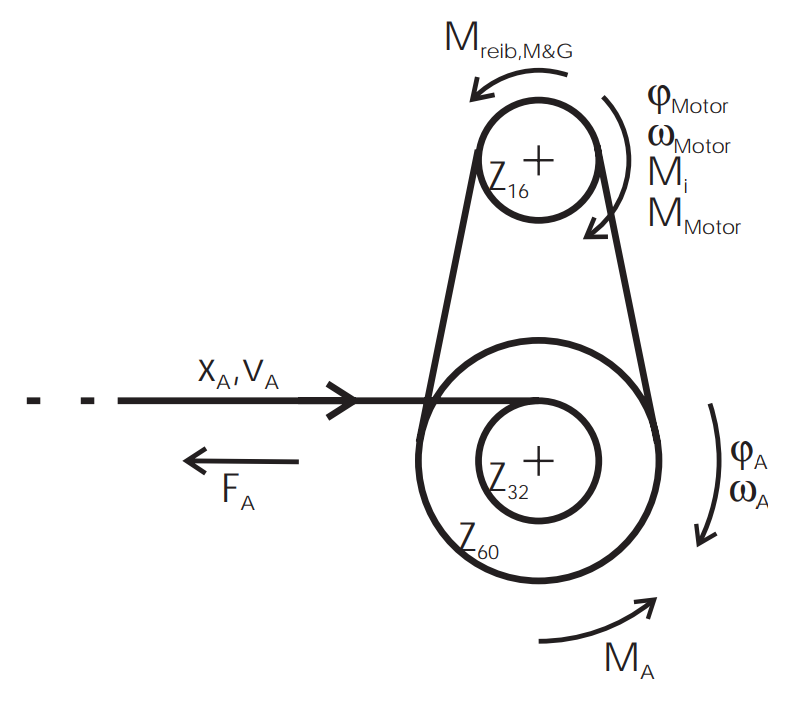
\includegraphics[width=0.50\textwidth]{Bilder/Modellierung/Getriebe.PNG}
	\caption{Getriebe \cite{franke}}
	\label{fig:Getriebe}
\end{figure}

Die Rotorbewegung des Motors wird über das in Abbildung \ref{fig:Getriebe} dargestellte Getriebe und das Antriebszahnrad auf den Zahnriemen weitergegeben. Auf Grund der hohen Steifigkeit des mit eingebetteten Stahlseilen unterstützten Riemens wird dieser wie in Apprich \cite{apprich} als unendlich starr angenommen, sodass die Verbindung von Motor und Schlitten ohne Federkopplung durch eine Übersetzungskonstante modelliert werden kann.
\[
	\dot{x} = K_G \cdot \omega_{Motor}
\]
 Die Übersetzungskonstante $K_G$ zwischen der Winkelgeschwindigkeit des Motors und der Schlittengeschwindigkeit wird über das Zahnverhältnis und den Antriebsradius berechnet.
\[
	K_G =  \frac{Z_{16}}{Z_{60}} \cdot r_{32} .
\]
Der Antriebsradius $r_{32}$ ist dabei der Abstand zwischen der neutralen Phase des Riemens und der Drehachse.


\section{Modellparameter}\label{sec:mparams}

Bevor die in dieser Arbeit verwendeten Parametersätze für Motor- und \spd-Modell vorgestellt werden, soll im folgenden Abschnitt zunächst ein Überblick über die Entwicklung der in den vergangenen Arbeiten verwendeten Modellparameter gegeben werden.  


\subsection{Begründeter Stand der Modellparameter}\label{subsec:paramshist}

Die für die Modellierung erforderlichen Systemparameter des Versuchsstands wurden erstmalig 1997 von Franke \cite{franke} durch Messungen identifiziert. Die Antriebseinheit aus Spannungs-Strom-Wandler, Motor, Getriebe und Riemen ist seitdem nicht verändert worden. Daher repräsentieren die von Franke \cite{franke} identifizierten Modellparameter in Bezug auf die Antriebseinheit weiterhin den aktuellen Stand (siehe \secref{subsec:motorparams})
   
Während zuvor noch ein Einfachpendel verwendet worden war, konstruierte Apprich \cite{apprich} 2009 erstmalig ein Doppelpendel für den Versuchsstand. Von den Änderungen betroffen war neben den Pendeln auch die Schlittenmasse, da auch der obere Teil des Schlittens neu konstruiert wurde. Die Modellparameter für die neuen Pendelstäbe wurden, anders als bei Franke \cite{franke}, nicht gemessen, sondern aus dem CAD-Modell abgeleitet. Dies betrifft die Massen, Trägheitsmomente, Längen und Schwerpunkte der beiden Stäbe. Die Masse des Schlittens wurde von Franke \cite{franke} übernommen. Durch Messungen wurden lediglich die viskose und trockene Reibung des Schlittens gegenüber den Schienen erneut identifiziert. 

Im selben Jahr wurde von Kämmerer \cite{kämmerer} die viskose Lagerreibung $d_1$ zwischen Stab 1 und dem Schlitten als fehlender Modellparameter durch Messungen ergänzt. Die viskose Lagerreibung $d_2$ zwischen Stab 1 und Stab 2 wurde rechnerisch bestimmt, da das Lager gegen Ende der Arbeit getauscht werden musste. Die viskose Dämpfung des Schlittens, die von Apprich \cite{apprich} zuvor gemessen worden war, wurde durch einen deutlich höheren Schätzwert ersetzt. Außerdem wurde erstmalig die Masse von Schlitten und Antrieb zu einer schlittenseitig wirkenden Gesamtmasse zusammengefasst und ebenfalls als Schätzwert ausgewiesen.

Die Reibwerte $d_1$ und $d_2$ wurden 2011 durch Kisner \cite{kisner} erneut bestimmt. Durch die \textit{Prediction-Error Minimization Method} aus der \textit{System Identification Toolbox} von \Matlab\ wurden die Parameter $d_1$ und $d_2$ so variiert, dass die quadratische Fehlersumme minimal wird. Als Fehler ist hierbei die Differenz zwischen den gemessenen und den vom Modell vorhergesagten zeitlichen Winkelverläufen $\varphi_1(t)$ und $\varphi_2(t)$ bei ruhendem Schlitten und frei gewählter Anfangsauslenkung zu verstehen. Für die Optimierung wurden zudem nicht näher beschriebene Anfangsschätzwerte für $d_1$ und $d_2$ gewählt. Es wird davon ausgegangen, dass es sich um Erfahrungswerte handelt, da sie einerseits nicht mit den zuletzt von Kämmerer \cite{kämmerer} bestimmten Werten übereinstimmen, jedoch andererseits zu guten Ergebnissen am Versuchsstand führten. Statt der optimierten Werte wurden in den Nachfolgearbeiten die Anfangsschätzwerte weiterverwendet. Der Reibwert $d_0$ der viskosen Schlittenreibung, der nicht Gegenstand der Optimierung war, wurde mit einem deutlich höheren Wert als bei Kämmerer \cite{kämmerer} angegeben. Da keine explizite Begründung vorliegt, wird von einem Erfahrungswert ausgegangen. Die zuvor von Kämmerer \cite{kämmerer} geschätzte effektive Gesamtmasse von Schlitten und Antrieb wurde nach unten korrigiert, wobei die Hintergründe für diesen Schritt ebenfalls nicht bekannt sind. Der neue Wert ist jedoch plausibel und wird daher ebenfalls als erfahrungsbasierter Schätzwert verstanden. Der ist in den weiteren Arbeiten nicht mehr verändert worden, sodass er als aktueller Stand zu betrachten ist. Bei Kisner \cite{kisner} wurde erstmalig auch eine Begrenzung der Stellkraft von $F_{\mrm{max}}=\valunit{400}{N}$ bezüglich des Schlittens angegeben, die als gegeben dokumentiert ist. 

2011 wurde außerdem von Noupa \cite{noupa} sowohl die viskose als auch die trockene Schlittenreibung gemessen, wobei besonders für die viskose Reibung eine hohe Richtungsabhängigkeit beobachtet wurde. Die gemessenen Werte wurden in den weiteren Arbeiten jedoch nicht weiter beachtet.

Auf Grund eines Austauschs des Lagers von Stab 2 wurde 2014 von Brehl \cite{brehl} eine erneute Identifikation der viskosen Dämpfungskonstanten $d_2$ messungsbasiert durchgeführt. Dabei wurden auch Länge und Masse von Stab 2 gemessen, womit ebenfalls das Massenträgheitsmoment neu berechnet wurde. In den Nachfolgearbeiten wurden jedoch nur die Dämpfungskonstante weiterverwendet, während für Länge, Masse und Trägheitsmoment weiterhin die CAD-Werte von Apprich \cite{apprich} verwendet wurden.  

Chang \cite{chang} konstruierte im Sommersemester 2019 ein neues Doppelpendel, wobei Schlitten und Antrieb nicht verändert worden sind. Die neuen Modellparameter wurden wieder aus dem CAD-Modell abgeleitet. Die Angabe des Schwerpunkts $s_2$ von Stab 2 scheint in der Ausarbeitung jedoch zu fehlen. Die Dämpfungskonstanten $d_1$ und $d_2$ wurden von den Vorgängern übernommen, da bei der Konstruktion die gleichen Rillenkugellager gewählt wurden wie bei Apprich \cite{apprich}. Für $d_1$ wurde der Schätzwert von Kisner \cite{kisner} und für $d_2$ der Messwert von Brehl \cite{brehl} übernommen, wobei in Changs Ausarbeitung versehentlich für beide Parameter Apprich \cite{apprich} als Quelle zitiert wird. Die viskose und die trockene Reibung des Schlittens wurden durch Messung selbst bestimmt. Wie bei Noupa \cite{noupa} wurde bei der viskosen Reibung eine auffällige Richtungsabhängigkeit festgestellt. Die Berücksichtigung der Richtungsabhängigkeit mit einer Vorsteuerung führte jedoch zu einer Verschlechterung des Systemverhaltens. Daher wurde schließlich die linksseitige Dämpfungskonstante für beide Seiten übernommen. Da das neu konstruierte Pendel noch nicht für die weiteren Bestandteile der Arbeit, wie die Auslegung der Regelung und deren Erprobung am Versuchsstand, zur Verfügung stand, wurde weiterhin auf die CAD-Werte von Apprich \cite{apprich} zurückgegriffen. Der Betrag der maximalen Stellkraft $F_{\mrm{max}}$ wurde zudem von dem von Kisner \cite{kisner} zuletzt genannten Wert von \valunit{400}{N} auf \valunit{421}{N} erhöht. Der neue Wert lässt sich rechnerisch nachvollziehen, wie \secref{subsec:motorparams} entnommen werden kann.

Im Rahmen einer Verifikation der von Chang \cite{chang} angegebenen Modellparameter für das neue Doppelpendel, wurden im Wintersemester 2019/2020 durch Ribeiro \cite{ribeiro} die Parameter aus dem CAD-Modell erneut abgeleitet. Da hierbei nicht genauer auf den Anlass der Neubestimmung eingegangen wurde, sich die neu bestimmten Parameter jedoch deutlich von den Vorherigen unterscheiden, wird angenommen, dass sich die von Chang \cite{chang} angegebenen Werte im Rahmen der Verifikation als fehlerbehaftet herausstellt hatten. 
Darüber hinaus wurde durch Messung die Reibung der Pendelgelenke identifiziert. Hierbei wurde neben der viskosen Reibung erstmalig auch die trockene Reibung in den Gelenken ermittelt. Die Parameter von Ribeiro \cite{ribeiro} zu den Pendelstäben sind somit aktueller Stand. Übernommen wurde weiterhin die von Kisner \cite{kisner} geschätzte Gesamtmasse mit Schlitten und Antrieb. Für die maximale Stellkraft wurde im Gegensatz zur Vorgängerarbeit Chang \cite{chang} statt \valunit{421}{N} wieder \valunit{400}{N} angenommen. Es wird vermutet, dass dadurch eine Stellkraftreserve für die Regelung vorgehalten werden sollte.


\subsection{Parameter des Motor-Modells}\label{subsec:motorparams}

Gemäß \secref{subsec:paramshist} werden die Modellparameter für das Motormodell Franke \cite{franke} entnommen. 

Die Steuerspannung $U_{\mrm{Steuer}}$ am Eingang des Spannungs-Strom-Wandlers darf maximal $\pm \valunit{10}{V}$ betragen. Ein Betrag größer als \valunit{10}{V} sollte vermieden werden, da sonst der Impulsstrom über den zulässigen Wert ansteigen und der Stromregler zerstört werden kann.

Die Verstärkung $K_{UI}$ des Spannungs-Strom-Wandlers kann durch ein Potentiometer bis zu einem Wert von etwa \valunit{2}{A/V} eingestellt werden, sodass mit der maximalen Steuerspannung der maximal zulässige Impulsstrom von \valunit{20}{A} erreicht wird. Die zuletzt dokumentierte Einstellung liegt bei
\[
	K_{UI} = \valunit{1,87}{\frac{A}{V}} \ .
\]
Der Wert beinhaltet bereits eine Idealisierung, da Messungen von Franke \cite{franke} gezeigt haben, dass die reale Verstärkung am Versuchsstand eine leichte Richtungsabhängigkeit bezüglich des Vorzeichens aufweist.

Die Zeitkonstante $T_{UI}$ wird als ausreichend klein angesehen, sodass die Dynamik des Wandlers vernachlässigt werden kann.

Alle weiteren verwendeten Parameter des Motormodells sind in \tabref{tab:motorparams} aufgeführt.

\begin{table}[h]
	\centering
	\caption{Parameter -- Motorsystem}
		\begin{tabular}[t]{cc} \
					Tabelle & Dummy \\
		\end{tabular}
	\label{tab:motorparams}
\end{table}


Mit der statischen Verstärkung zwischen Eingang $U_{\mrm{Steuer}}$ und Ausgang $F$
\begin{align}
	K_{\mrm{MotorGain}} = K_{UI} \cdot K_I \cdot \frac{1}{K_G} \cdot \frac{1}{r_{32}} = \valunit{42,075}{\frac{N}{V}}
	\label{eq:motgain}
\end{align}
lässt sich die maximale Stellkraft
\begin{align}
	F_{\mrm{max}} = U_{\mrm{Steuer, max}} \cdot K_{\mrm{MotorGain}} = \valunit{420,75}{N}
\end{align}
berechnen, wobei $K_{UI} = \valunit{1,87}{A/V}$ ist.
Für $K_{UI \mrm{, max}} = \valunit{2}{A/V}$ läge die maximale Stellkraft bei $F_{\mrm{max}} = \valunit{450}{N}$.



\subsection{Parameter des Schlittendoppelpendels}\label{subsec:spdparams}

Ausgehend von \secref{subsec:paramshist} werden in dieser Arbeit drei Parametersätze angelegt \siehe{\tabref{tab:spdparams}}.
Dies ermöglicht einen Vergleich der unterschiedlichen Systeme hinsichtlich des Systemverhaltens und der Stabilisierbarkeit.

Aufgrund der Neukonstruktion des \dpd s und dabei aufgetretener Schwierigkeiten in der Regelung ist ein Vergleich zum vorigen System von Interesse.
Die Parameter der alten Konstruktion werden mit \qq{Apprich09} bezeichnet, obwohl hier auch neu bestimmte Werte von Kisner \cite{kisner} und Brehl \cite{brehl} (Reibung und Schlittenträgheit) enthalten sind.
Der zweite Parametersatz \qq{Chang19} stellt die Daten der Ausarbeitung von \cite{chang} dar, in welcher die Neukonstruktion stattfand. 
Da diese erst in der nächsten Arbeit (Ribeiro \cite{ribeiro}) in Betrieb genommen wurde und dort sowohl die CAD-Parameter erneut bestimmt als auch die Reibungsparameter identifiziert wurden, werden die Werte \qq{Ribeiro20} als korrekte Parameter des neukonstruierten \dpd s betrachtet.

\begin{table}[htbp]
	\centering
	\caption{Parameter -- \spds}
		\begin{tabular}{lcc|lll}
			\toprule
			Bezeichnung	&	Symbol	&	Einheit	&	Apprich09	&	Chang19	&	Ribeiro20	\\
			\midrule
			Masse des Schlittens	&	$m_0$	&	\unit{kg}	&	16,5	&	16,5	&	16,5	\\
			Masse des ersten Pendels	&	$m_1$	&	\unit{kg}	& 0,615	&	0,329	&	0,8534	\\
			Masse des zweiten Pendels	&	$m_2$	&	\unit{kg}	&	0,347	&	0,3075	&	0,3957	\\
			Trägheitsmoment des ersten Pendels	&	$J_1$	&	\unit{kg \,m^2}	&	0,00647 &	0,01457	&	0,01128	\\
			Trägheitsmoment des zweiten Pendels	&	$J_2$	&	\unit{kg \,m^2}	&	0,00407	&	0,00334	&	0,003343	\\
			Länge des ersten Pendels	&	$l_1$	&	\unit{m}	&	0,2905	&	0,325	&	0,282	\\
			Länge des zweiten Pendels	&	$l_2$	&	\unit{m}	&	0,3388	&	0,305	&	0,280	\\
			Schwerpunkt des ersten Pendels	&	$s_1$	&	\unit{m}	&	0,0775	&	0,1425	&	0,09373	\\
			Schwerpunkt des zweiten Pendels	&	$s_2$	&	\unit{m}	&	0,146	&	0,114254	&	0,114254	\\
			Viskose Dämpfung des Schlittens	&	$d_0$	&	\unit{\frac{N s}{m}}	&	17	&	17,6	&	17	\\
			Viskose Dämpfung des ersten Pendels	&	$d_1$	&	\unit{\frac{N m s}{rad}}	&	0,0091	&	0,005	&	0,00768	\\
			Viskose Dämpfung des zweiten Pendels	&	$d_2$	&	\unit{\frac{N m s}{rad}}	&	0,0006905	&	0,005	&	0,000285	\\
			\crb\ des Schlittens	&	\Fco	&	\unit{N}	&	16,232	&	17,5	&	13,43	\\
			\crb\ des ersten Pendels	& \Mceo	&	\unit{Nm}	&	0	&	0,0538	&	0,0538	\\
			\crb\ des zweiten Pendels	& \Mczo	&	\unit{Nm}	&	0	&	0,0000912	&	0,0000912	\\
			Erdbeschleunigung	&	$g$	&	\unit{\frac{m}{s^2}}	&	9,81	&	9,81	&	9,81	\\
			\bottomrule
		\end{tabular}
	\label{tab:spdparams}
\end{table}

Es wird somit im Folgenden zwischen den \qq{alten Parametern} (\texttt{Apprich09}) und den \qq{neuen Parametern} (\texttt{Ribeiro20}) unterschieden.
Der größte Unterschied zwischen beiden Systemen ist die \crb\ in den Pendelgelenken, die zusätzlich zur viskosen Reibung erstmals bei Ribeiro \cite{ribeiro} bestimmt wurde.
Da bei der Neukonstruktion die Messsignalübertragung zur Vermeidung einer Kabelaufwickelung über einen Schleifring realisiert wurde, besteht die Vermutung, dass dieser für die erhöhte \crb\ verantwortlich ist. 
Dies macht das System bereits um einen sehr kleinen Arbeitsbereich nichtlinear, was die Regelung erschwert.

Für die Skalierungsparameter \xopth, \pheth\ und \phzth\ der \crb\ \siehe{\secref{sec:crb}} wird jeweils 0,01 angenommen.



\section{Aufbau des Simulationsmodells}

In dieser Arbeit wird das \dpds\ rein simulativ betrachtet.
Das Simulationsmodell wird im Vergleich zu Vorgängerarbeiten wesentlich systematischer und detaillierter aufgebaut.
Dadurch sind umfangreiche und automatisierte Tests möglich, mit denen das System umfassend untersucht werden kann.

Besonders wird in dieser Arbeit Wert auf einen strukturierten, modularen Aufbau gelegt.
Dies soll flexible Änderungen am System, wie \zB Systemparameter oder Reglerparameter ermöglichen.
Von der Berechnung der \bwgl\ über die Parametrisierung des Systems bis zur Reglerberechnung kann das Modell vollständig und konsistent initialisiert werden.
Außerdem soll dadurch die Nutzbarkeit und Wiederverwendbarkeit in zukünftigen Arbeiten gewährleistet sein.

Das Simulationsmodell voriger Arbeiten wie \cite{chang} ist nur wenig strukturiert aufgebaut, enthält Redundanzen und viele fest-kodierte Parameter.
Es wird daher lediglich zur Orientierung verwendet.
Hart-kodierte Parameter werden in dieser Arbeit vermieden, sodass jeder Parameter bei der \init\ geändert werden kann (ohne das \sm-Modell ändern zu müssen).
Auch Gleichungen können variabel ausgelegt werden, was durch die symbolische Schreibweise von \ml\ ermöglicht wird.
Code-Dopplungen werden vermieden. 
Die gesamte \init\ ist stark funktionalisiert.
Dadurch wird sichergestellt, dass Änderungen nur an einer Stelle vorgenommen werden müssen und automatisch direkt an allen entsprechenden Stellen angepasst werden.

Die \sm-Modelle und \ml-Funktionen zur Modellierung des Systems und \init\ des Simulationsmodells befinden sich im Ordner \texttt{Modell}. 


\subsection{Aufbau in \Simulink}

\subsubsection{Subsysteme}
In \sm\ lassen sich sogenannte \emph{Subsysteme} erstellen, um ein Simulationsmodell übersichtlicher zu gestalten.
Diese Subsysteme (im Folgenden auch Module genannt) lassen sich zudem als Datei externalisieren (\emph{Referenced Subsystem}), wodurch sie einerseits seperat bearbeitet werden können und andererseits an mehreren Stellen modular wiederverwendet werden können.
Somit wird lediglich in der obersten Schicht (die Testebene) ein \sm-\emph{Model} verwendet.

In dieser Arbeit werden immer Module erstellt, sofern es sinnvoll erscheint.
Dadurch wird das Gesamtsystem übersichtlich gehalten und kann sehr flexibel modifiziert werden.
Die einzelnen Module (wie \zB Motor, Gesamtmodell, \zsr) stellen zudem wiederverwendbare Teile dar und können so an verschiedenen Stellen im Projekt eingebaut werden, aber möglicherweise auch am \sm-Modell des Versuchsstandes zum Einsatz kommen.
So könnte relativ einfach derselbe Regler an dem echten und dem simulierten System eingesetzt und verglichen werden.

\subsubsection{Maske}
Bei Subsystemen kann eine sogenannte \emph{Maske} eingerichtet werden, wodurch Parameter übergeben werden können.
In deren Abhängigkeit können in einem Subsystem auch initialisierende Berechnungen durchgeführt werden.

Grundsätzlich können in \sm\ alle Variablen aus dem globalen \ml-Workspace verwendet werden, was allerdings fehleranfällig ist.
Geschickter ist es, dem Simulationsmodell eine einzige Variable vom Typ \texttt{struct} zu übergeben, in der alle Parameter vorhanden sind.
So werden jedem Modul über die jeweilige Maske nur genau die Parameter übergeben, von denen es abhängt.
Dadurch bleibt der Gesamtaufbau modularer und strukturierter.

\subsubsection{Scopes und ToWorkspace}
Um die Signalverläufe direkt zu untersuchen, werden an allen wichtigen Stellen in den Simulationsmodellen \emph{Scopes} installiert.
So lässt sich das Systemverhalten oder Probleme in der Regelung schnell und einfach analysieren.
Oft werden Scopes mit mehreren Eingängen verwendet, um Signale besser vergleichen zu können.

Für alle Variablen, die später in \ml\ für weitere Auswertungen zur Verfügung stehen sollen, werden \emph{ToWorkspace}-Blöcke verwendet.
Diese geben die Daten an die Ausgabevariable \texttt{out}.

Für die Screenshots werden diese Blöcke meist aus Übersichtsgründen entfernt.


\subsection{\Simulink\ Module und Modelle}

\subsubsection{Motor.slx}
Das Motormodell wird \secref{sec:mot} entsprechend als Modul implementiert \siehe{\figref{fig:simmot}}.
Eingangsgröße ist die Steuerspannung sowie die Schlittengeschwindigkeit, da sich daraus die Induktionsspannung ergibt.
Ausgangsgröße ist die Kraft, die am Schlitten wirkt.
Der V/A Wandler wird als Subsystem implementiert und gibt den Motorstrom aus \siehe{\figref{fig:simva}}.
Die Berechnung der Strombegrenzung \siehe{\secref{subsec:dcMotor}} wird als \emph{matlabFunction} realisiert.
Dabei werden die Signale \texttt{satState\_w} (falls die Sättigungsdrehzahl erreicht ist) und \texttt{satState\_I} (falls der Sollstrom nicht erreicht werden kann) gesetzt und können später analysiert werden.
Die Tiefpass-Charakteristik der Induktivität wird mit dem \mrm{PT_1}-Glied \eqref{eq:UI} dargestellt.

\begin{figure}
	\centering
		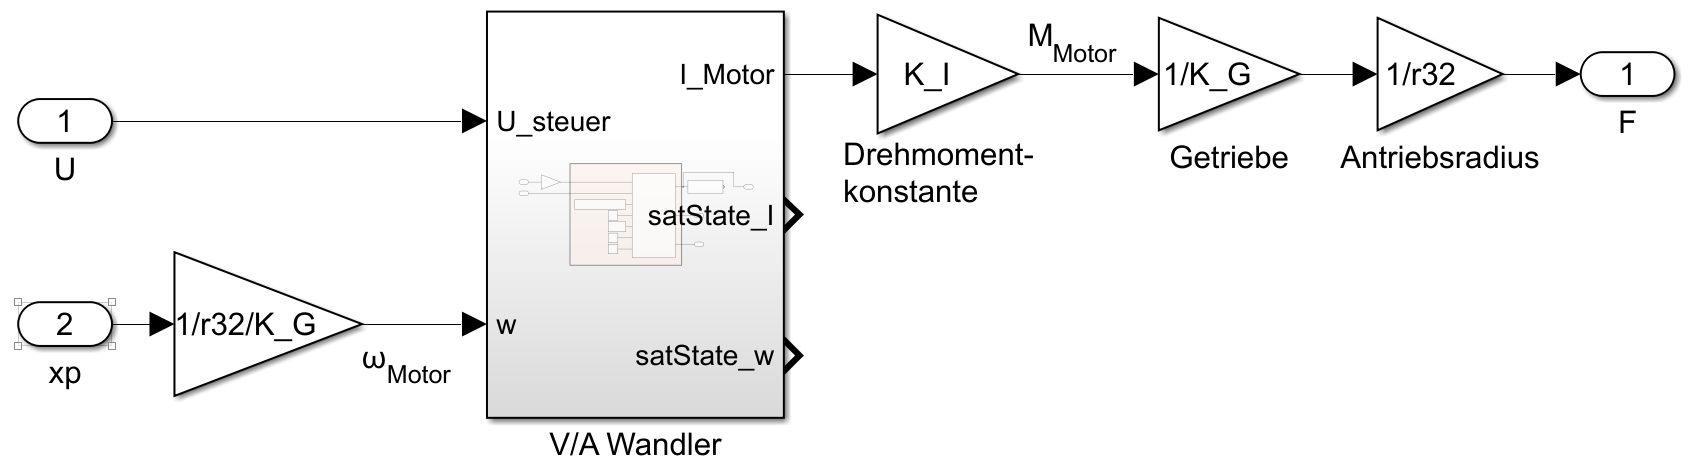
\includegraphics[scale=0.6]{Bilder/Simulink/motor.PNG}
	\caption{Motormodell in \sm}
	\label{fig:simmot}
\end{figure}

\begin{figure}
	\centering
		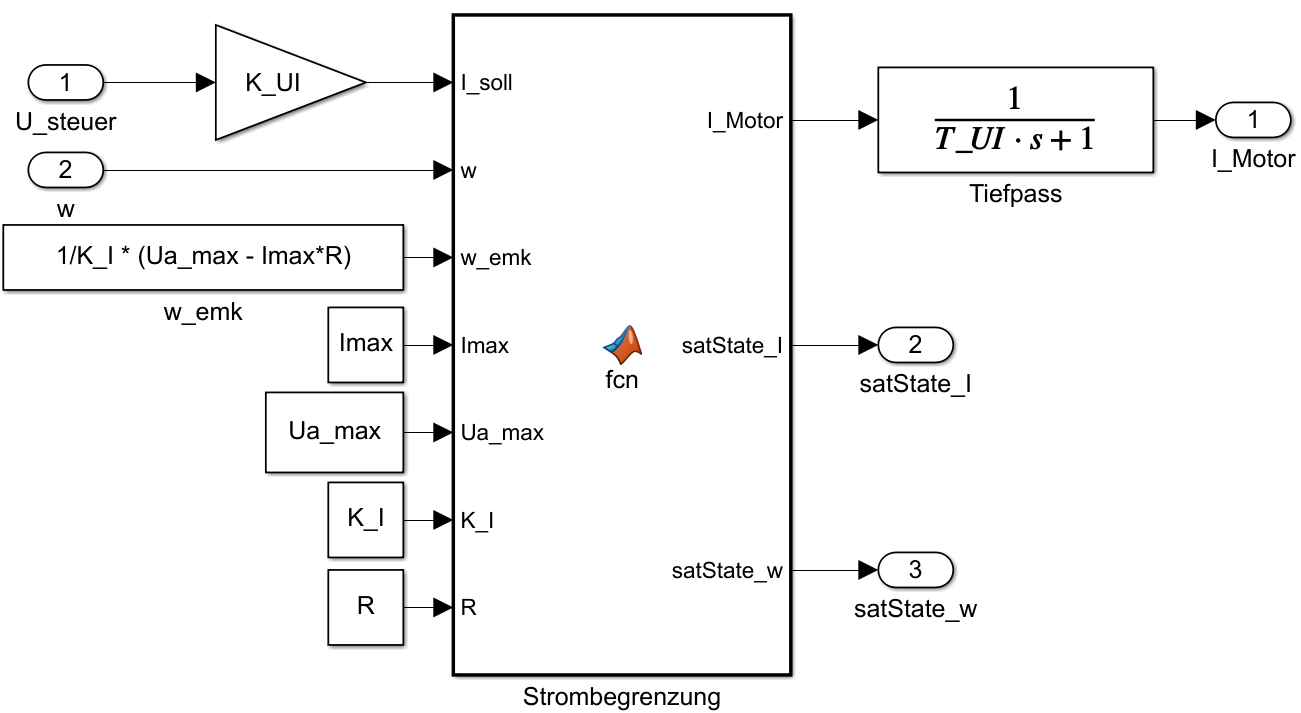
\includegraphics[scale=0.5]{Bilder/Simulink/va_wandler.PNG}
	\caption{V/A Wandler in \sm}
	\label{fig:simva}
\end{figure}

\subsubsection{SchlittenPendel.slx}
Das \zrm\ des \spds s wird mit einer \emph{S-Function} dargestellt.
Die zugehörige \ml-Datei \texttt{SchlittenPendelFunc.m} wird automatisch bei der \init\ erstellt \siehe{\secref{subsec:init}}.
Lediglich die Anfangswerte werden über die Simulationsparameter übergeben.

\subsubsection{Gesamtmodell.slx}\label{sec:gesamtslx}
Dieses Modul stellt das gesamte Modell dar und fasst die beiden vorigen Module zusammen \siehe{\figref{fig:simges}}.
Die Eingangsspannung wird an den Motor gegeben und dessen Ausgang $F$ ist die Schnittstelle zum \sdpd.
Die Schlittengeschwindigkeit wird zum Motor zurückgeführt, da durch diese die Motordrehzahl bestimmt wird.
\begin{figure}
	\centering
		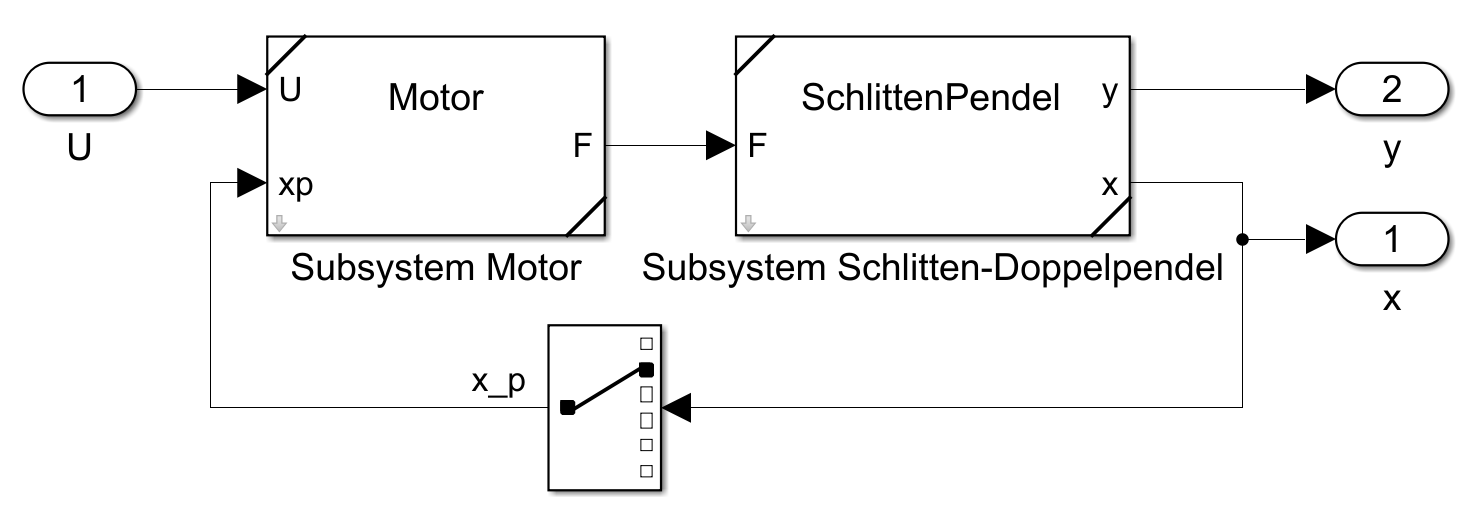
\includegraphics[scale=0.4]{Bilder/Simulink/gesamtmodell.PNG}
	\caption{Gesamtmodell in \sm}
	\label{fig:simges}
\end{figure}

\subsubsection{Gesamtmodell\_Test.slx}
Dies ist ein \sm-Modell und bindet das Gesamtmodell-Modul ein.
Auf dieses können testweise verschiedene Eingangsverläufe gegeben werden, um das Systemverhalten auf Plausibilität zu überprüfen, beispielsweise:
\begin{itemize}
	\item Keine Spannung, aber Anregung durch Anfangsauslenkung
	\item Konstante Spannung
	\item Sinusförmige Spannung
\end{itemize}
Da die durchgeführten Tests am Modell plausible Ergebnisse zeigen, wird im Folgenden von der Korrektheit des Simulationsmodells ausgegangen.


\subsection{Parameter}

Größere zusammenhängende Parameterdaten werden als Datei \bzw Funktion ausgelagert, um eine einfache Austauschbarkeit zu erreichen.
Die drei Parametersätze des \spd s \siehe{\tabref{tab:spdparams}} sowie die Motorparameter befinden sich im Ordner \texttt{Modellparameter}.


\subsection{Initialisierung}\label{subsec:init}

\texttt{Init.m}
%Wie schon in \secref{subsec:bwgl} erwähnt, werden die \bwgl\ des \spds\ symbolisch errechnet.
%Die Gleichungen werden in \texttt{SchlittenPendelSymF.m} definiert und die Lösungen der drei \bwgl\ bestimmt.


\subsection{Auswertung}

Nach einer Simulation ist es nützlich, die wesentlichen Ergebnisse direkt ablesen zu können (\zB ob der Schlitten außerhalb der Begrenzung war oder ob der Motor in Sättigung war).
Außerdem wird eine Plot-Funktion implementiert, die die wichtigsten Verläufe darstellt.
Um das Verhalten des \dpd s besser interpretieren zu können, wird zudem eine Animationsfunktion erstellt, die direkt das Pendelverhalten visualisiert.
Die entsprechenden \ml-Funktionen sind im Ordner \texttt{Auswertung} vorhanden.

\subsubsection{plot}

\subsubsection{animate}



\subsection{Weitere \Matlab-Funktionen}

Weitere Informationen und Kommentare finden sich auch meist in den \ml-Funktionen selbst.


\texttt{SchlittenPendelNLZSR.m}

\texttt{SchlittenPendelSymA.m}

\texttt{SchlittenPendelSymF.m}

\texttt{SchlittenPendelRuhelagen.m}

\texttt{SchlittenPendelFunc.m}